% Source-faithful schematic draft: 2004 Hunan Arts Q22, PDF p.2 (printed p.177).
% Source ID: src-69c1d502b386b3e69e4b98d9f5500c36d4b278d52aa54448a71182edf7c03358
% Source SHA-256: dc0e39533bc2dd37833ae2dc4bdb93e31a39d08808c842611458bf0b844aaeed
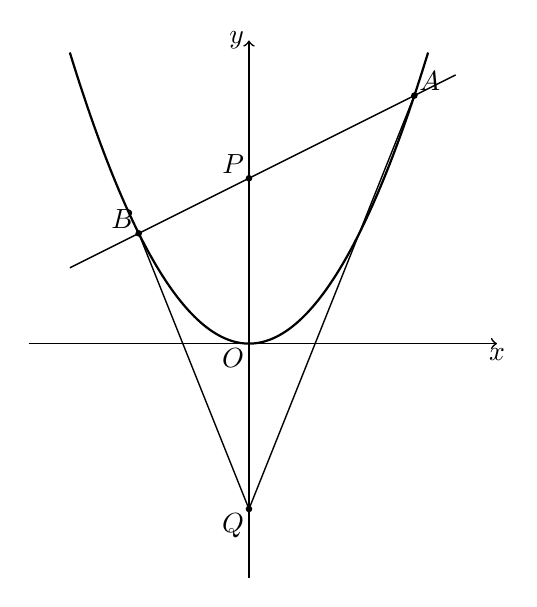
\begin{tikzpicture}[line width=0.6pt,scale=0.35,every node/.style={inner sep=1.5pt}]
  % Axes
  \draw[->] (-8, 0) -- (9, 0) node[below] {$x$};
  \draw[->] (0, -8.5) -- (0, 11) node[left] {$y$};
  \node[below left] at (0, 0) {$O$};

  % Parabola x^2 = 4y => y = x^2 / 4
  \draw[thick,domain=-6.5:6.5,samples=60,smooth] plot (\x, {0.25*\x*\x});

  % Points P(0, 6) and Q(0, -6)
  \coordinate (P) at (0, 6);
  \coordinate (Q) at (0, -6);
  \fill (P) circle (0.12) node[above left] {$P$};
  \fill (Q) circle (0.12) node[below left] {$Q$};

  % Points A(6, 9) and B(-4, 4) on parabola and line y = 0.5x + 6
  \coordinate (A) at (6, 9);
  \coordinate (B) at (-4, 4);
  \fill (A) circle (0.12) node[above right] {$A$};
  \fill (B) circle (0.12) node[above left] {$B$};

  % Secant line AB passing through P
  \draw[line width=0.55pt] (-6.5, 2.75) -- (7.5, 9.75);

  % Lines QA and QB
  \draw[line width=0.5pt] (Q) -- (A);
  \draw[line width=0.5pt] (Q) -- (B);
\end{tikzpicture}
